%%%%%%%%%%%%%%%%%%%%%%%%%%%%%%%%%%%%%%%%%%%%%%%%%%%%%%%%%%%%%%%%%%%%%
% LaTeX Template: Project Titlepage Modified (v 0.1) by rcx
%
% Original Source: http://www.howtotex.com
% Date: February 2014
% 
% This is a title page template which be used for articles & reports.
% 
% This is the modified version of the original Latex template from
% aforementioned website.
% 
%%%%%%%%%%%%%%%%%%%%%%%%%%%%%%%%%%%%%%%%%%%%%%%%%%%%%%%%%%%%%%%%%%%%%%

\documentclass[12pt, UKenglish]{report}
\usepackage[a4paper]{geometry}
\usepackage[myheadings]{fullpage}
\usepackage{fancyhdr}
\usepackage{lastpage}
\usepackage{graphicx}
\usepackage{wrapfig}
\usepackage{subcaption}
\usepackage{setspace}
\usepackage{booktabs}
\usepackage[T1]{fontenc}
\usepackage[font=small, labelfont=bf]{caption}
\usepackage{fourier}
\usepackage[protrusion=true, expansion=true]{microtype}
\usepackage[UKenglish]{babel}
\usepackage{sectsty}
\usepackage{url, lipsum}
\usepackage{tgbonum}
\usepackage[colorlinks = true,
            linkcolor = blue,
            urlcolor  = blue,
            citecolor = blue,
            anchorcolor = blue]{hyperref}
\usepackage{xcolor}
\usepackage{isodate}
\usepackage{enumitem}
\usepackage{wrapfig}
\usepackage[backend=bibtex]{biblatex}
\usepackage{mdframed}
\usepackage{verbatimbox}

\usepackage{listings, color}    
\usepackage{textcomp}
\usepackage{fancyvrb}
\usepackage{verbatim}

\newcommand{\HRule}[1]{\rule{\linewidth}{#1}}
\onehalfspacing
\setcounter{tocdepth}{5}
\setcounter{secnumdepth}{5}

%-------------------------------------------------------------------------------
% HEADER & FOOTER
%-------------------------------------------------------------------------------
%\pagestyle{fancy}
%\fancyhf{}
%\setlength\headheight{15pt}
%\fancyhead[L]{Student ID: 1034511}
%\fancyhead[R]{Anglia Ruskin University}
%\fancyfoot[R]{Page \thepage\ of \pageref{LastPage}}
%-------------------------------------------------------------------------------
% TITLE PAGE
%-------------------------------------------------------------------------------

\begin{document}
{\fontfamily{cmr}\selectfont
\title{ \normalsize \textsc{}
		\\ [2.0cm]
		\HRule{0.5pt} \\
		\LARGE \textbf{\uppercase{Project Documentation}
		\HRule{2pt} \\ [0.5cm]
		\normalsize \vspace*{5\baselineskip}}
		}

\author{
		Michael Trapp\\
		Department of Earth Science and Engineering\\
		Imperial College London}

\maketitle
\tableofcontents
\newpage

%-------------------------------------------------------------------------------
% Section title formatting
\sectionfont{\scshape}
%-------------------------------------------------------------------------------

%-------------------------------------------------------------------------------
% BODY
%-------------------------------------------------------------------------------

\section{Highlights}
\bigbreak

\bigbreak
\noindent{\color{blue}\textbf{\printdate{2019-7-01}}}
There is an {\color{red} error} with the simulations. The \texttt{Y2D} code will compile, but the visualised output in \texttt{paraview} consists of random stripes and patterns.

\bigbreak
\noindent{\color{blue}\textbf{\printdate{2019-7-18}}}
The material parameters and simulation parameters are wrong. They need to be adjusted using formulas. This did not remove the visualisation errors, however.

\bigbreak
\noindent{\color{blue}\textbf{\printdate{2019-7-25}}} - {\color{blue}\textbf{\printdate{2019-7-28}}}
A \texttt{c++} file to generate the y file directly is now created, though still some bugs. However, the geometry still needs to be created separately independently. The approach is not scientifically relevant and was therefore abandoned.

\bigbreak
\noindent{\color{blue}\textbf{\printdate{2019-7-29}}}
Breakthrough during session with supervisor: The nodes for each element were listed in the wrong rotational order (counter-clockwise / clockwise), this lead to negative area, which lead to negative mass, which lead to code compilation errors. The error was perhaps produced by using \texttt{GiD} or \texttt{Y2D} code with the wrong operating system.

\bigbreak
\noindent{\color{blue}\textbf{\printdate{2019-8-02}}}
The simulations are running now, and showing good geometry. However, the body interactions are completely wrong. For example, a steel ball deforms on contact with the glass plies, instead of breaking it.

\bigbreak
\noindent{\color{blue}\textbf{\printdate{2019-8-07}}}\\
Legacy \texttt{vtk} file output works. \\
\texttt{VTK} \texttt{XML} file format output works, but only for \texttt{ascii} encoding.

\bigbreak
\noindent{\color{blue}\textbf{\printdate{2019-8-19}}}\\
\texttt{VTK} \texttt{XML} \texttt{b64} encoding looks relatively genuine, although there are still errors.


\newpage
\section{Project Specific Updates}
\noindent{\color{blue}\textbf{\printdate{2019-7-01}}-\textbf{\printdate{2019-7-10}}}
Time has been invested to understand the software \texttt{GiD} and the \texttt{FEMDEM} theory. The supervisors are busy or away on conferences and don't react to emails.

\bigbreak
\noindent{\color{blue}\textbf{\printdate{2019-7-10}}}
No \texttt{2D} simulation is running. Out of frustration, as no supervisor is reacting, a one-week 'vacation' was taken to concentrate on getting any simulation running. During 'vacation', the student misses a very important meeting with a mechanical engineer professor from Imperial who is researching in the field of modelling glass breakage.

\bigbreak
\noindent{\color{blue}\textbf{\printdate{2019-7-17}}}
Simple \texttt{2D} impact tests were conducted. The geometry is illustrated in Fig. \ref{fig:initgeom}. However, these tests are not running. The correct geometry is not able to be visualized. Instead, some random patterns and lines appear when trying to visualize using \texttt{paraview}.

\begin{wrapfigure}{R}{0.3\textwidth}
	\centering
	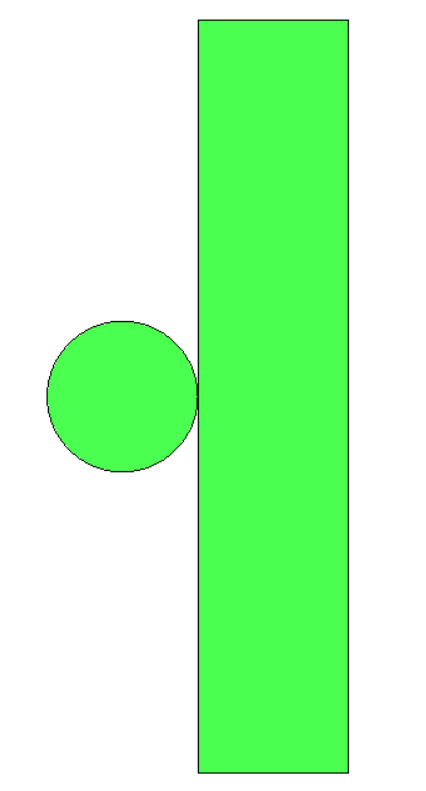
\includegraphics[width=0.3\textwidth]{initial_geometry.PNG}
	\caption{Simple test geometry ('geometry 1').}
	\label{fig:initgeom}
\end{wrapfigure}

\begin{figure}[!h]
	\centering
	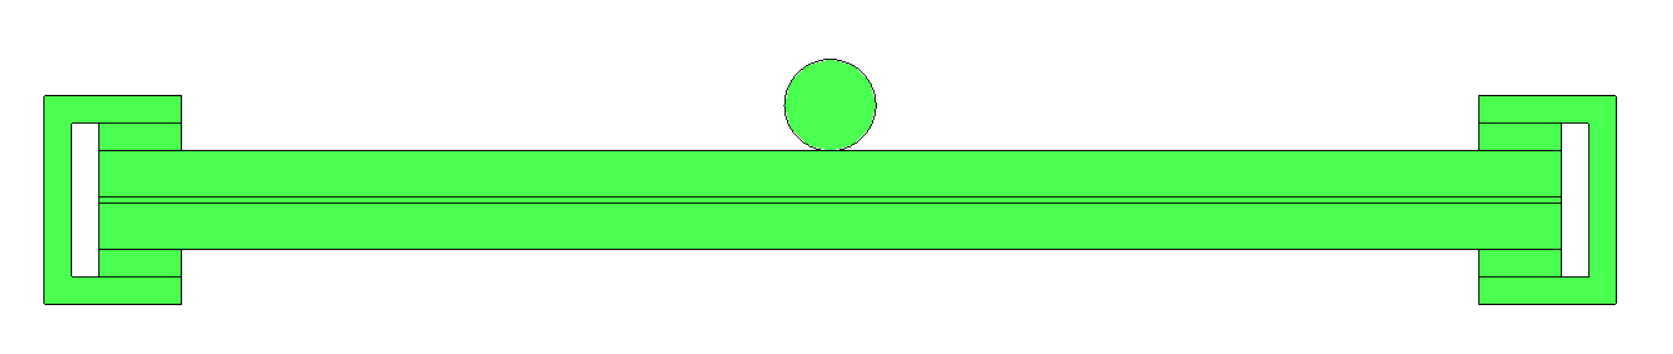
\includegraphics[width=0.8\textwidth]{geometry2.PNG}
	\caption{A more sophisticated test geometry ('geometry 2').}
	\label{fig:geometry2}
\end{figure}

\bigbreak
\noindent{\color{blue}\textbf{\printdate{2019-7-18}}}
Meeting with supervisors. The parameters are wrong, as they need to be determined by use of formulas. For this purpose, it is necessary to introduce additional parameters, such as total minimum element volume, minimum edge, critical time step of glass, steel, pvb, etc - these must be read from the program GUI. Using the formulas via an external excel spreadsheet, the simple simulation (\texttt{geometry1}) is now running, provisionally using material for rock (as opposed to glass/steel/pvb).

\bigbreak
\noindent{\color{blue}\textbf{\printdate{2019-7-19}}}
Another geometry is adduced, see Fig. \ref{fig:geometry2}. Simulation using this new geometry, along with proper material data failed. The supervisors are not available right now. This prompts the following conduction of systematic tests, always using the excel spreadsheet:

\begin{enumerate}[topsep=0pt,itemsep=-1ex,partopsep=1ex,parsep=1ex,label= {\color{blue}\textbf{test\arabic*}\,\,}]
    \item geometry 1, rock
    \item geometry 1, glass/steel
    \item geometry 2, fine mesh, rock
    \item geometry 1, glass
    \item geometry 1, steel
    \item geometry 1, glass, high penalty factor $p$
    \item geometry 1, steel, high penalty factor $p$
    \item geometry 2, fine mesh, glass
    \item geometry 2, fine mesh, steel
    \item geometry 2, fine mesh, pvb
    \item geometry 2, coarse mesh, rock
\end{enumerate}

\textbf{Conclusions from the tests}:

\begin{enumerate}[topsep=0pt,itemsep=-1ex,partopsep=1ex,parsep=1ex,label=\Alph*)]
    \item The issue is not with geometry 1, material rock or material steel.
    \item \textbf{Materials glass and pvb} needs be perhaps be reconsidered, as tests with these materials have consistently not been successful.
    \item \textbf{Geometry 2} needs to perhaps be reconsidered. The fact that test 11 and test 3 fail implies that some parameters for geometry 2 are wrong.
\end{enumerate}

\bigbreak
\noindent{\color{blue}\textbf{\printdate{2019-7-22}}} All tests are repeated. Due to simulation errors continuing to appear, another approach is necessary. The supervisors are still busy. 

\bigbreak
As the \texttt{GiD UI} may be the source of the problem, it was attempted to create a \texttt{Y2D} file from scratch using \texttt{C++} programming language. This would incorporate the formulas from the excel spreadsheet. Implementation of the Y file generation code led to the encounter of several problems:

\begin{enumerate}
    \item Problems with the generation of the mesh. A mesh algorithm could be written if information was present on how the GiD program generates the mesh. A pseudo code or technique in the manuals could not be found. It may not be productive to apply any random mesh generation method - although tempting.
    \item Problems with the parameters. Parameters such as '\texttt{/YD/YDE/I1ELTY}', '\texttt{/YD/YDC/ICFMTY}', '\texttt{/YD/YDP/D1PBIF}', etc. etc. are not explained in the entire Munjiza literature. This makes it difficult to manually assign parameters. Perhaps the FEMDEM code may permit to draw conclusions on these parameters. It is unlikely that pontential comments could give explanations on the usability.
\end{enumerate}

\bigbreak
A new approach is to now use the GiD customisation system, which may be automisable to the point where calculation of the \texttt{Y} file from the GiD folder leads to good data. Example files on this matter were already provided by the supervisors as early as {\textbf{\printdate{2019-6-20}}}, but only now is the content understandable/tangible.

\bigbreak
\noindent{\color{blue}\textbf{\printdate{2019-7-23}}}
Paraview is now setup on HPC. A windows batch file has been created to run the program. However, it is unclear how the y file is generated via command line. The \texttt{HPC} questions were mostly answered. The files and folders can now be sent to the \texttt{HPC} system and back.

\bigbreak
\noindent{\color{blue}\textbf{\printdate{2019-7-24}}}
An Ubuntu batch file is now created. It reads in user variables, which contain the user specific paths and names. The command from which \texttt{GiD} created the \texttt{Y} file from a \texttt{.dat} (?) file is unclear. The \texttt{.ym} files are successfully generated locally via invoking the \texttt{Y2D} \texttt{bin} files (\texttt{Yf}, \texttt{m2vtu} and \texttt{m2vtu\_crack}) locally. The \texttt{.vtu} and \texttt{.vtu\_crack} files are not generated, however, because a library is missing (libvtk5.8.0.so.common). Local calculation would be faster than invoking the HPC server every time. Trying to set up automatic calculation is the best approach since this enables quick tests with many parameters. This is to the opnion of the author the best approach at the moment.

\bigbreak
\noindent{\color{blue}\textbf{\printdate{2019-7-25}}} - {\color{blue}\textbf{\printdate{2019-7-28}}}
A \texttt{c++} file to generate the y file directly is now created, though still some bugs.

\bigbreak
\noindent{\color{blue}\textbf{\printdate{2019-7-29}}}
\textbf{BREAKTHROUGH} after several hours during session with supervisors: The nodes for each element were listed in the wrong order (counter-clockwise / clockwise), this lead to negative area, which lead to negative mass, which lead to code compilation errors. The discrepancy (wrong rotation) may be produced due to importing the geometry from Autocad, although \texttt{geometry1} was entirely generated with GiD and also produced errors.

\bigbreak
\noindent{\color{blue}\textbf{\printdate{2019-7-30}}}
The \texttt{Yf} code needs to be recompiled. However, there are errors when calling the make file. These errors were fixed during the \texttt{HPC} walk-in clinic session today. It was also attempted to set up \texttt{VTK 5.8} version locally for easier and faster testing. However, this proved too difficult. The \texttt{HPC} system stays the only option. \texttt{GMESH} is now being set up to generate a mesh, which makes using \texttt{GiD} completely obsolete. \texttt{GMESH} will give full control over the information which node is assigned to which element and material. \texttt{GMESH} can be incorporated into the \texttt{c++} code due to the existance of a \texttt{GMESH} \texttt{c++} \texttt{API}.

\bigbreak
\noindent{\color{blue}\textbf{Objectives}}\newline
The goal is now to produce simulations, introduce joint elements between elements of different materials, update the version of \texttt{VTK} and introduce a new elastomer material law.

\bigbreak
\noindent{\color{blue}\textbf{\printdate{2019-07-31}}}
The \texttt{GMESH} \texttt{API} could not be incorporated. It was attempted to write a separate \texttt{c++} file which would generate a \texttt{.geo} file, which in turn would be able to be compiled by \texttt{gmesh}. It would still need to be considered how to again read the data again and generate the \texttt{y} file for the \texttt{y2D} program. The whole approach was abandoned, as it is not scientifically relevant.\\

During a meeting with the supervisor, he generated a simple \texttt{y} file with \texttt{GiD}. The new objectives are to include joint elements between different materials, update the file output and write a new elastomer law. The \texttt{y} file can be used to test modifications of the code.

\bigbreak
\noindent{\color{blue}\textbf{\printdate{2019-08-01}}}
The \texttt{Y2D} code was extensively studied and code to generate simple \texttt{VTK} legacy files was written, however not tested yet.

\bigbreak
\noindent{\color{blue}\textbf{\printdate{2019-08-02}}}
Code to generate \texttt{VTK} \texttt{xml} files was written. The code to generate \texttt{VTK} legacy files was tested. The \texttt{VTK} legacy file is written nicely (according to formatting rules) but there is an error when reading. During testing with a \texttt{.y} input file with a setup of two 'rectangles' moving apart (total nodes: $8$), it was discovered that the total number of nodes has mistakenly increased (to $20$). Using the same input file, the original code was adduced and it was discovered that the number of nodes still mistakenly increased. The code was compiled on the \texttt{ubuntu} 16.0 subsystem on windows. In the meanwhile, a new remote operating system surface with \texttt{ubuntu} 14.0, \texttt{GiD} 10.0.9 and \texttt{paraview} 5.4.1 was set up for the student ('ese-pollux'). The \texttt{Y2D} code compilation generated the wrong number of nodes here as well.

\begin{figure}[!h]
	\centering
	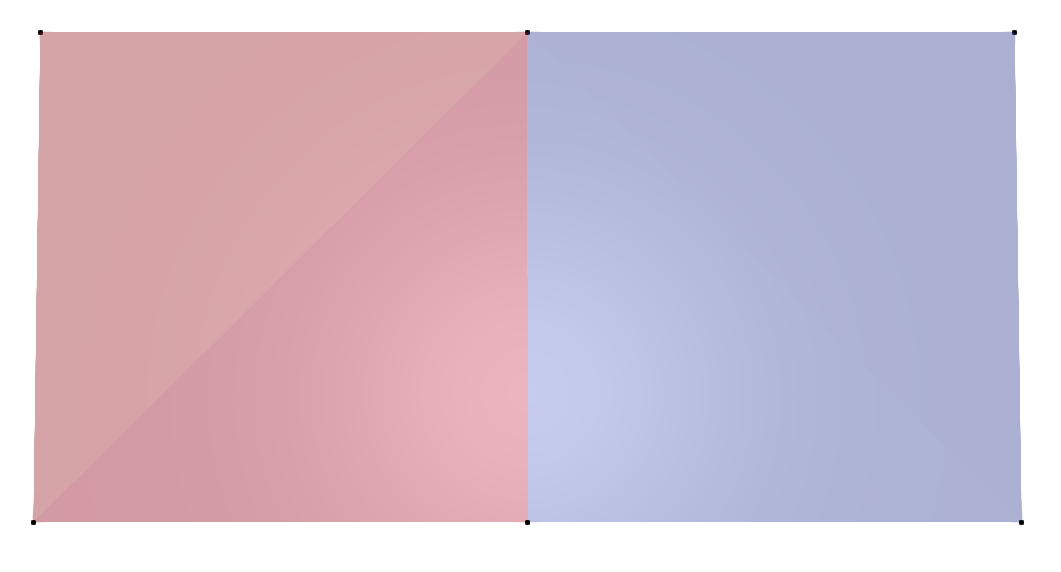
\includegraphics[width=0.8\textwidth]{rectangles.PNG}
	\caption{Simulation of two rectangles drifting apart, at initial time, with nodes visible; number of nodes = 8}
	\label{fig:geometry2}
\end{figure}

\begin{figure}[!h]
	\centering
	
\includegraphics[width=0.8\textwidth]{endstate.PNG}
	\caption{Simulation of two rectangles drifting apart, at final time. The area between the rectangles at the top border is magnified; still number of nodes = 8}
	\label{fig:geometry2}
\end{figure}

\begin{figure}[!h]
	\centering
	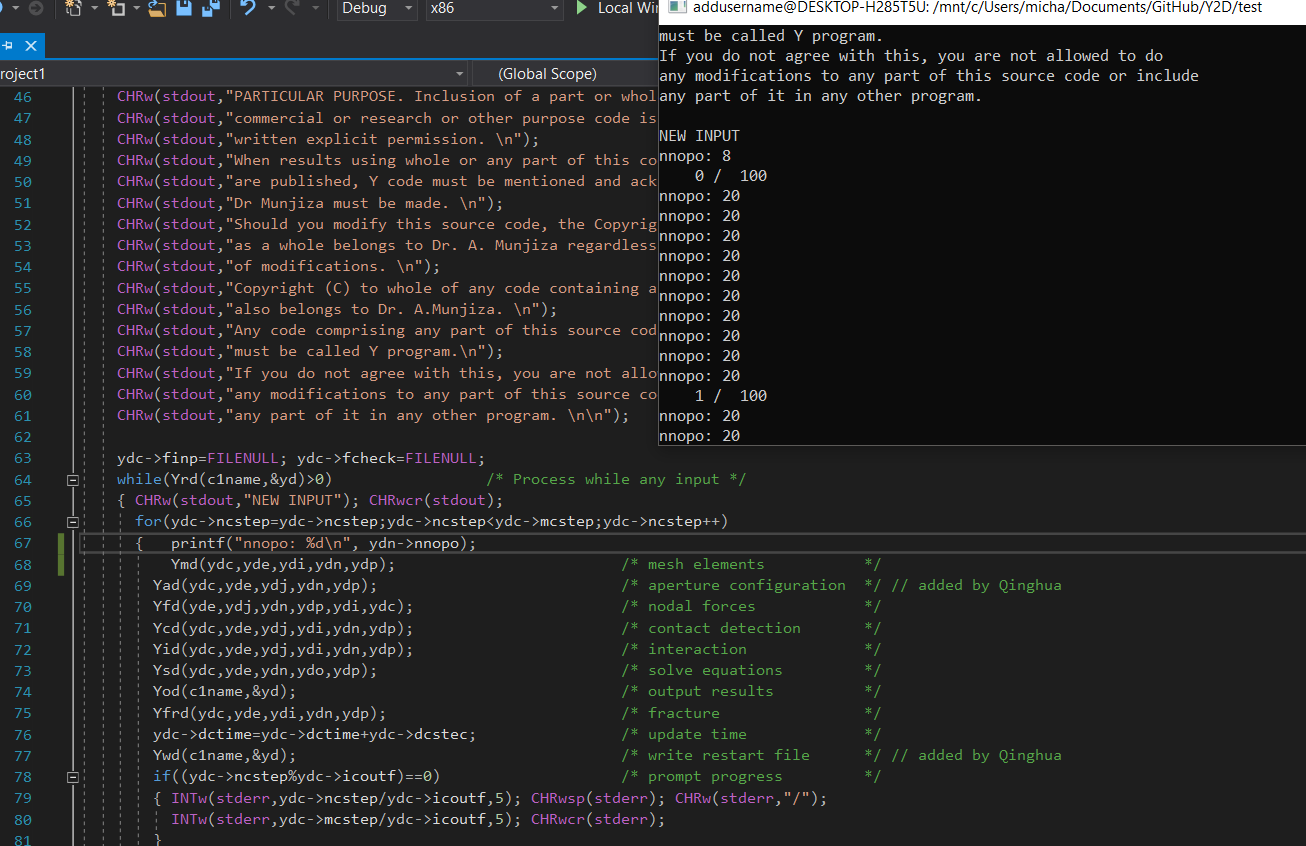
\includegraphics[width=0.8\textwidth]{nodeschange.PNG}
	\caption{Code screenshot of executing the original code and cmd ouput, only with one added print statement, using the \texttt{.y} input file where 2 rectangles moving apart. The (actual) number of nodes \texttt{nnopo} changes from $nnopo=8$ to $nnopo=20$, the (actual) number of elements \texttt{nelem} changes from $nelem=4$ to $nelem=14$. Is the entire code wrong?}
	\label{fig:geometry2}
\end{figure}

\bigbreak
\noindent{\color{blue}\textbf{\printdate{2019-08-03}}} - {\color{blue}\textbf{\printdate{2019-08-05}}}
The supervisor created a folder "/data" in the newly created remote server \url{ese-pollux.ese.ic.ac.uk}. However, the folder is in the supervisor's directory and cannot be accessed. In the meanwhile, a drawing has been created (Fig. \ref{fig:node_ele_drawn}) which shows how the original code produces the wrong nodes and elements. The self-created \texttt{.vtu} output file is also given below.

\bigbreak
The folder was in some root directory and could be accessed. The folder contains the \texttt{full} code, i.e. the code for all three executables (\texttt{Yf}, \texttt{m2vtu}, \texttt{m2vtu\_crack}. The way the student generated the \texttt{vtk} files now appears to be completely wrong. They are generated by use of \texttt{vtk} libraries, instead of by use of the \texttt{printf( )} command. The '\texttt{printf( )} - approach' is now abandonned and effort is now spent on the '\texttt{vtk} - approach'.

\begin{figure}[!h]
	\centering
	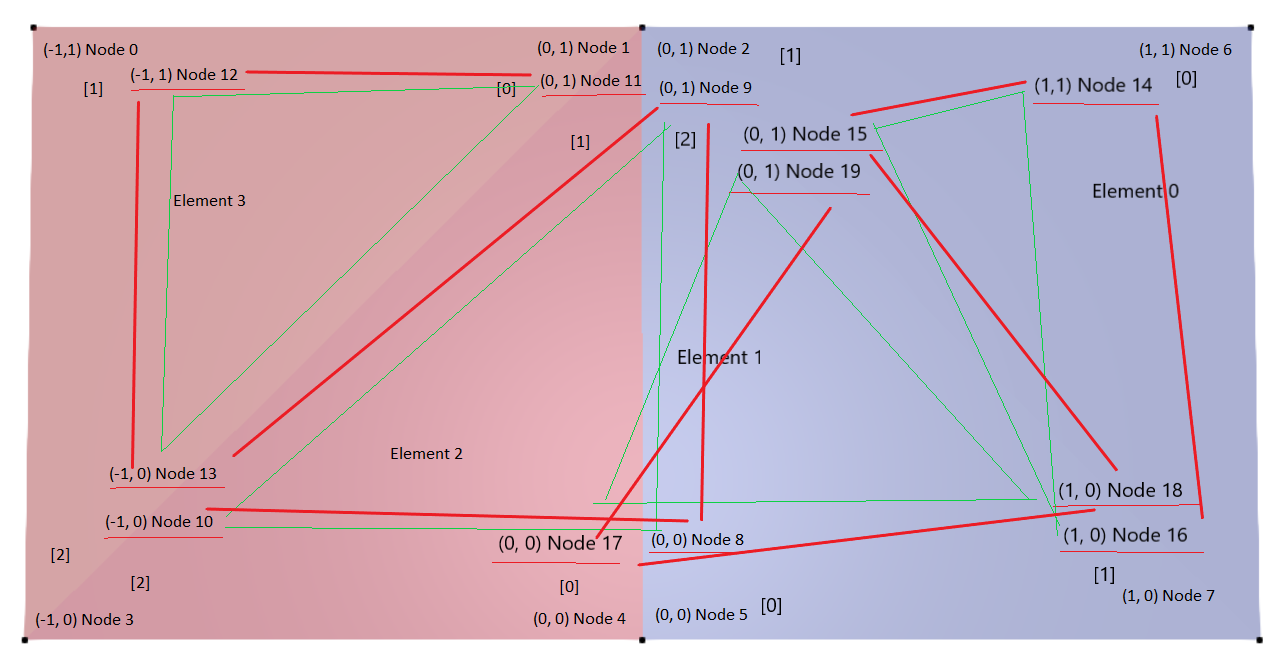
\includegraphics[width=0.8\textwidth]{rectangles_drawn.PNG}
	\caption{Nodes and Elements created using original code, visualised by use of print statements}
	\label{fig:node_ele_drawn}
\end{figure}

\verbfilebox[\tiny]{test_int0.vtu}\fbox{\theverbbox}

\bigbreak
\noindent{\color{blue}\textbf{\printdate{2019-08-06}}}
The approach by the student was right - the \texttt{vtk} libraries should not be used if possible. New program code has been implemented to only write the unique nodes and elements, and also to remove elements which have 2 equal nodes - these elements are not triangles. These details are thought to produce the errors in \texttt{paraview}. In the example of the two rectangles moving apart, now only 4 elements are nicely written to the \texttt{vtk} file. However, when opening the \texttt{vtk} legacy file with \texttt{paraview}, there is an error that there is an issue with the dataset size. The format information for \texttt{vtk} legacy files needs to be researched again. Perhaps there is an issue with the format.

\bigbreak
The code was developed in windows due to \texttt{visual studio} being available as a nice editor, even though the code is only compilable using the \texttt{ubuntu} subsystem. The code was secure copied to the remote \texttt{ese-pollux} for testing, and some \texttt{-c99} issues emerged, such as errors of loop declarations. Even though all errors could be fixed, the program still does not compile. The error was localized to be in an independent section of the code, not in the code written by the student. Specifically, the error appears just before entering the data reading function \texttt{Yrd}. An email was not written yet, as perhabs investigating a little further will quickly fix the issue.

\bigbreak
The \texttt{HPC} clinic session today was fruitful inasmuch as keys and aliases were generated for the remotes and the putty options (as advised by Geraldo Fiorino Neto who set up the \texttt{ese-pollux} depository could potentially be replaced by \texttt{bash} commands.

\bigbreak
\noindent{\color{blue}\textbf{\printdate{2019-08-07}}} The day was spent on generating \texttt{paraview} complient \texttt{vtk} \texttt{vtu} files. Both options - legacy and \texttt{xml} work flawlessly now. Coordination with the supervisor is necessary to specify exactly which output is necessary, i.e. besides points and elements, e.g. forces, stress and such.

\bigbreak
\noindent{\color{blue}\textbf{\printdate{2019-08-08}}} 
It was attempted to encode the data to base 64 (b64). Opening the file in paraview, however, resulted in errors.

\bigbreak
\noindent{\color{blue}\textbf{\printdate{2019-08-09}}}
The student came down with a painful eye disease, therefore work had to be interrupted.

\bigbreak
\noindent{\color{blue}\textbf{\printdate{2019-08-12}}}
Due to the persistent eye disease, not much work could be done. Before encoding the data to b64, apparently encoding to b2 (binary) is necessary. The most useful, although still cryptic, information could be found \href{http://www.earthmodels.org/software\/vtk-and-paraview/vtk-file-formats}{here}.
The problem is that the format is not specified clear enough. Is double encoding, i.e. b10 -> b2 -> b64 necessary? The header needs to be 4 byte long, but which base does this length refer to?\\
The supervisors cannot help.

\bigbreak
\noindent{\color{blue}\textbf{\printdate{2019-08-13}}}
The b2 encoding was misunderstood. The encoding is for single bytes, not \texttt{ints} (whole numbers). But even after the corrections the program is not working.

\bigbreak
\noindent{\color{blue}\textbf{\printdate{2019-08-14}}}
Maybe the step from creating vtk legacy askii to vtk xml b64 encoded files was too big. Many other formats were attempted to be created, but only askii formats work. Binary and b64 formats consistently fail. Just like with the simulations there might be some platform issues when converting binaries, for example.

\bigbreak
\noindent{\color{blue}\textbf{\printdate{2019-08-15}} - \color{blue}\textbf{\printdate{2019-08-16}}}
A function is written which saves the int32 to chars and then sends the char array to the encoder function, which encodes 3 bytes a time. The question was asked on  \href{https://stackoverflow.com/questions/57539806/how-do-i-encode-a-float32-to-b64-in-c}{on stackoverflow}.

\bigbreak
\noindent{\color{blue}\textbf{\printdate{2019-08-17}}} The problem is shifting a \texttt{float32}, \texttt{int32} to a \texttt{char} array to prepare for the \texttt{b64} encoding. There are several methods of doing so. It has been attempted to use type casting such as \texttt{bytes = (UCHR *)&header;} to transfer the \texttt{int} to a \texttt{char} array. The results seemed extremely promising, and the encoding looked valid. However, the output changes every time after compilation, and \texttt{paraview} returns errors upon opening the encoded file.

\bigbreak
\noindent{\color{blue}\textbf{\printdate{2019-08-19}}} Another tactic may be to use \texttt{unions}, classes with variables of different data types which point to the same memory. However, this approach seems not to be feasible, as dynamic float arrays need to be 'converted'. Ideas like \href{https://stackoverflow.com/questions/50087561/initializing-dynamic-array-of-unions-in-c}{this} one are unlikely to be fruitful.

\bigbreak
After reassigning the data to a new \texttt{CHR} array with \texttt{malloc} and \texttt{memcpy}, the encoding works.

\bigbreak
\noindent{\color{blue}\textbf{\printdate{2019-08-20}}}
Meeting with supervisor. There need to be some flags, as the joint elements do not always have 3 nodes (they are not always triangles). This issue has been encountered earlier and led to an incredible amount of confusion. Presumably, this only involves setting flags for the element inter-connectivity and the element types, but the focus should now be on finishing the report in time.

\bigbreak
\noindent{\color{blue}\textbf{\printdate{2019-08-19}} - \printdate{2019-08-23}} Time was invested in writing a detailed and comprehensible report.

\newpage
\section{Things I Need Help with and my Plan to Resolve}
{\color{blue}\textbf{\printdate{2019-07-21}}}

\bigbreak
\noindent\textbf{Parameters}\\
What are these parameters?:
\begin{enumerate}[topsep=0pt,itemsep=-1ex,partopsep=1ex,parsep=1ex,label=\Alph*)]
    \item \texttt{/ YD / YDC / ICFMTY}
    \item \texttt{/ YD / YDC / ICIATY}
\end{enumerate}

{\color{green}SOLVED}

\bigbreak
\noindent\textbf{HPC walk-in clinic \textbf{\printdate{2019-07-23}}}
        \begin{enumerate}[topsep=0pt,itemsep=-1ex,partopsep=1ex,parsep=1ex,label=\Alph*)]
            \item remove standard output and error from home directory
            \item make qsub.sh and qstat.sh working from local directory, for both ubuntu subsystem and git bash
            \item why do the paths work without variable but not with variables in bash, e.g. \$variable/qsub vs. bin/qsub
            \item scp secure copy does "setup2d/setup2d" -> I am confusing a subdirectory, how to copy directory into directory?
            \item .bashrc and .bash\_profile are broken in git bash, /esc/skil is empty;	where to get a fresh copy
            \item use paraview in hpc, should be all set up
            \item copy and paste with nano and vim
        \end{enumerate}
        
{\color{green}SOLVED}

\bigbreak
\noindent\textbf{Simulations}\\
Modify material parameters for geometry 1, e.g. penalty factor, buffer size. Studying the \texttt{2D} \texttt{Y} Code might give answers as to why the calculation breaks. An attempt is being made to write a \texttt{C++} program to generate a Y file. This could eventually then be integrated in the automation system to generate the Y file, automatically send it to the \texttt{HPC} system, calculate it and automatically analyse it using \texttt{Paraview}.
{\color{green}SOLVED}

\bigbreak
\noindent{\color{blue}\textbf{\printdate{2019-07-22}}} Feedback on approaches.
{\color{green}SOLVED}

\bigbreak
\noindent{\color{blue}\textbf{\printdate{2019-07-23}}} How to calculate the y file with windows batch file?
{\color{green}SOLVED}

\bigbreak
\noindent{\color{blue}\textbf{\printdate{2019-07-24}}} As the supervisors are away, there are no new revelations about what could have gone wrong with these simple simulations. An email was sent to the supervisors concerning questions about GiD:

\begin{enumerate}[topsep=0pt,itemsep=-1ex,partopsep=1ex,parsep=1ex,label=\Alph*)]
    \item What is the command line command to convert files in a GiD folder to a \texttt{Y} file?
    \item Do I need to create a new problem type instead of \texttt{B2D}?
    \item What is the \texttt{.dat} file and do I need it if I have y files?
\end{enumerate}
{\color{green}SOLVED}

\bigbreak
\noindent{\color{blue}\textbf{\printdate{2019-08-03}}}
There is an error with the node count in the \texttt{Y2D} program - the number of nodes of two rectangles drifting apart increases from $8$ to $20$, seemingly randomly. A non-buggy version of the code would be helpful, even if less developed. Otherwise time will be spent on fixing the errors.

{\color{green}SOLVED}: Supervisor said this is right, this is the creation of joint elements. Though why are they combined with the original elements, i.e. how to distinguish the two?

\bigbreak
What use is \texttt{GiD} on the \texttt{Linux} remote server? Command line arguments of calculating \texttt{.y} files from \texttt{.dat} files are not known to me (cannot be found in any manual), and a \texttt{GiD} \texttt{GUI} would surely not exist on \texttt{Linux}.

{\color{green}SOLVED}: Geraldo helped, gui works, {\color{blue}\textbf{\printdate{2019-08-06}}}: Santiago (\texttt{HPC} \texttt{RCS}) showed a way of enabling \texttt{X11} on \texttt{ese-pollux} remote server - thus making \texttt{putty} potentially superfluous. 

\bigbreak
\noindent{\color{blue}\textbf{\printdate{2019-08-03}}}
How to access the original elements and nodes - without the joint elements? Is this even necessary for the creation of the \texttt{vtk} files? It will be vital for the creation of joint elements between materials. {\color{green}SOLVED}: by the student. It is necessary to specify all points and elements, including the joint element ones in the output file. \texttt{paraview} knows what to do with them. No need to separate. 

\bigbreak
\noindent{\color{blue}\textbf{\printdate{2019-08-14}}}
Why is the encoding not working: What is the exact format of the vtk xml b64 encoded file?

%\input{tinhw.tex}

%-------------------------------------------------------------------------------
% REFERENCES
%-------------------------------------------------------------------------------
\newpage
\section*{References}

%[2]John W. Eaton, David Bateman, Sren Hauberg, Rik Wehbring (2015). GNU
%Octave version 4.0.0 manual: a high-level interactive language for numer-
%ical computations. Available: http://www.gnu.org/software/octave/doc/
%interpreter/. 
}
\end{document}

%-------------------------------------------------------------------------------
% SNIPPETS
%-------------------------------------------------------------------------------

%\begin{figure}[!ht]
%	\centering
%	\includegraphics[width=0.8\textwidth]{file_name}
%	\caption{}
%	\centering
%	\label{label:file_name}
%\end{figure}

%\begin{figure}[!ht]
%	\centering
%	\includegraphics[width=0.8\textwidth]{graph}
%	\caption{Blood pressure ranges and associated level of hypertension (American Heart Association, 2013).}
%	\centering
%	\label{label:graph}
%\end{figure}

%\begin{wrapfigure}{r}{0.30\textwidth}
%	\vspace{-40pt}
%	\begin{center}
%		\includegraphics[width=0.29\textwidth]{file_name}
%	\end{center}
%	\vspace{-20pt}
%	\caption{}
%	\label{label:file_name}
%\end{wrapfigure}

%\begin{wrapfigure}{r}{0.45\textwidth}
%	\begin{center}
%		\includegraphics[width=0.29\textwidth]{manometer}
%	\end{center}
%	\caption{Aneroid sphygmomanometer with stethoscope (Medicalexpo, 2012).}
%	\label{label:manometer}
%\end{wrapfigure}

%\begin{table}[!ht]\footnotesize
%	\centering
%	\begin{tabular}{cccccc}
%	\toprule
%	\multicolumn{2}{c} {Pearson's correlation test} & \multicolumn{4}{c} {Independent t-test} \\
%	\midrule	
%	\multicolumn{2}{c} {Gender} & \multicolumn{2}{c} {Activity level} & \multicolumn{2}{c} {Gender} \\
%	\midrule
%	Males & Females & 1st level & 6th level & Males & Females \\
%	\midrule
%	\multicolumn{2}{c} {BMI vs. SP} & \multicolumn{2}{c} {Systolic pressure} & \multicolumn{2}{c} {Systolic Pressure} \\
%	\multicolumn{2}{c} {BMI vs. DP} & \multicolumn{2}{c} {Diastolic pressure} & \multicolumn{2}{c} {Diastolic pressure} \\
%	\multicolumn{2}{c} {BMI vs. MAP} & \multicolumn{2}{c} {MAP} & \multicolumn{2}{c} {MAP} \\
%	\multicolumn{2}{c} {W:H ratio vs. SP} & \multicolumn{2}{c} {BMI} & \multicolumn{2}{c} {BMI} \\
%	\multicolumn{2}{c} {W:H ratio vs. DP} & \multicolumn{2}{c} {W:H ratio} & \multicolumn{2}{c} {W:H ratio} \\
%	\multicolumn{2}{c} {W:H ratio vs. MAP} & \multicolumn{2}{c} {\% Body fat} & \multicolumn{2}{c} {\% Body fat} \\
%	\multicolumn{2}{c} {} & \multicolumn{2}{c} {Height} & \multicolumn{2}{c} {Height} \\
%	\multicolumn{2}{c} {} & \multicolumn{2}{c} {Weight} & \multicolumn{2}{c} {Weight} \\
%	\multicolumn{2}{c} {} & \multicolumn{2}{c} {Heart rate} & \multicolumn{2}{c} {Heart rate} \\
%	\bottomrule
%	\end{tabular}
%	\caption{Parameters that were analysed and related statistical test performed for current study. BMI - body mass index; SP - systolic pressure; DP - diastolic pressure; MAP - mean arterial pressure; W:H ratio - waist to hip ratio.}
%	\label{label:tests}
%\end{table}%\documentclass{article}
%\usepackage[utf8]{inputenc}

%\title{Weekly Report template}
%\author{gandhalijuvekar }
%\date{January 2019}

%\begin{document}

%\maketitle

%\section{Introduction}

%\end{document}


%\begin{enumerate}[topsep=0pt,itemsep=-1ex,partopsep=1ex,parsep=1ex,labe%l=\Alph*)]
%    \item total minimum element volume
%    \item total minimum edge
%    \item total real simulation time
%    \item critical time step glass
%    \item critical time step steel
%    \item critical time step pvb
%    \item critical time step rock
%    \item number of output files
%    \item projectile mesh size
%    \item ply mesh size
%    \item interlayer mesh size
%\end{enumerate}